\documentclass[a4paper,12pt]{extarticle}
\usepackage[utf8x]{inputenc}
\usepackage[T1,T2A]{fontenc}
\usepackage[russian]{babel}
\usepackage{hyperref}
\usepackage{indentfirst}
\usepackage{listings}
\usepackage{color}
\usepackage{here}
\usepackage{array}
\usepackage{multirow}
\usepackage{graphicx}

\usepackage{caption}
\renewcommand{\lstlistingname}{Программа} % заголовок листингов кода

\bibliographystyle{ugost2008ls}

\usepackage{listings}
\lstset{ %
extendedchars=\true,
keepspaces=true,
language=C,						% choose the language of the code
basicstyle=\footnotesize,		% the size of the fonts that are used for the code
numbers=left,					% where to put the line-numbers
numberstyle=\footnotesize,		% the size of the fonts that are used for the line-numbers
stepnumber=1,					% the step between two line-numbers. If it is 1 each line will be numbered
numbersep=5pt,					% how far the line-numbers are from the code
backgroundcolor=\color{white},	% choose the background color. You must add \usepackage{color}
showspaces=false				% show spaces adding particular underscores
showstringspaces=false,			% underline spaces within strings
showtabs=false,					% show tabs within strings adding particular underscores
frame=single,           		% adds a frame around the code
tabsize=2,						% sets default tabsize to 2 spaces
captionpos=t,					% sets the caption-position to top
breaklines=true,				% sets automatic line breaking
breakatwhitespace=false,		% sets if automatic breaks should only happen at whitespace
escapeinside={\%*}{*)},			% if you want to add a comment within your code
postbreak=\raisebox{0ex}[0ex][0ex]{\ensuremath{\color{red}\hookrightarrow\space}},
texcl=true,
inputpath=listings,                     % директория с листингами
}

\usepackage[left=2cm,right=2cm,
top=2cm,bottom=2cm,bindingoffset=0cm]{geometry}

%% Нумерация картинок по секциям
\usepackage{chngcntr}
\counterwithin{figure}{section}
\counterwithin{table}{section}

%%Точки нумерации заголовков
\usepackage{titlesec}
\titlelabel{\thetitle.\quad}
\usepackage[dotinlabels]{titletoc}

%% Оформления подписи рисунка
\addto\captionsrussian{\renewcommand{\figurename}{Рисунок}}
\captionsetup[figure]{labelsep = period}

%% Подпись таблицы
\DeclareCaptionFormat{hfillstart}{\hfill#1#2#3\par}
\captionsetup[table]{format=hfillstart,labelsep=newline,justification=centering,skip=-10pt,textfont=bf}

%% Путь к каталогу с рисунками
\graphicspath{{fig/}}


\begin{document}	% начало документа

% Титульная страница
\begin{titlepage}	% начало титульной страницы

	\begin{center}		% выравнивание по центру

		\large Санкт-Петербургский Политехнический Университет Петра Великого\\
		\large Институт компьютерных наук и технологий \\
		\large Кафедра компьютерных систем и программных технологий\\[6cm]
		% название института, затем отступ 6см
		
		\huge Верификация и анализ программ\\[0.5cm] % название работы, затем отступ 0,5см
		\large Отчет по лабораторной работе №1\\[0.1cm]
		\large Построение поведенческой модели программы по структурной модели\\[5cm]

	\end{center}


	\begin{flushright} % выравнивание по правому краю
		\begin{minipage}{0.25\textwidth} % врезка в половину ширины текста
			\begin{flushleft} % выровнять её содержимое по левому краю

				\large\textbf{Работу выполнил:}\\
				\large Зорин А.Г.\\
				\large {Группа:} 23541/3\\
				
				\large \textbf{Преподаватель:}\\
				\large Ицыксон В.М.

			\end{flushleft}
		\end{minipage}
	\end{flushright}
	
	\vfill % заполнить всё доступное ниже пространство

	\begin{center}
	\large Санкт-Петербург\\
	\large \the\year % вывести дату
	\end{center} % закончить выравнивание по центру

\thispagestyle{empty} % не нумеровать страницу
\end{titlepage} % конец титульной страницы

\vfill % заполнить всё доступное ниже пространство


% Содержание
% Содержание
\renewcommand\contentsname{\centerline{Содержание}}
\tableofcontents
\newpage




\section{Цель работы}

Построить поведенческую модель программы по структурной модели. Программа должна принимать на вход файл с исходным кодом, написанном на языке программирования Java и выдавать в качестве результата файл с описанием поведенческой модели для всех методов, описанных в поданном файле. Вбранные модели следующие:
\begin{itemize}
\item \textbf{Структурная модель:} абстрактное синтаксическое дерево (AST)
\item \textbf{Поведенческая модель:} граф потока управления (CFG)
\end{itemize}

\section{Теоретическая информация}

\subsection{AST}

Абстрактное синтаксическое дерево --- помеченное ориентированное дерево, в котором внутренние вершины сопоставлены с операторами языка программирования, а листья --- с соответствующими операндами. Таким образом, листья являются пустыми операторами и представляют только переменные и константы. 

Синтаксические деревья используются в парсерах для промежуточного представления программы между деревом разбора и структурой данных, которая за этим используется в качестве внутреннего представления в компиляторе или интерпретаторе компьютерной программы для оптимизации и генерации кода. 

\subsection{CFG}

Граф потока управления --- множество всех возможных путей исполнения программы, представленное в виде графа. 

В графе потока управления каждый узел графа соответствует базовому блоку --- прямолинейному участку кода, не содержащему в себе ни операций передачи управления, ни точек, на которые управление передается из других частей программы. Имеется лишь два исключения:
\begin{itemize}
\item точка, на которую выполняется переход, является первой инструкцией в базовом блоке
\item базовый блок завершается инструкцией перехода
\end{itemize}

\section{Ход выполнения работы}

Общий план выполнения работы:
\begin{itemize}
\item Получение AST из исходного кода на Java
\item Построение CFG из AST
\item Экспорт CFG в PNG
\end{itemize}

\subsection{Взаимодействие с AST}

Для построения AST из исходного кода была использована часть из IDE Intellij Idea. Данная часть позволяет построить и модифицировать AST. Для того, чтобы обойти все интересующие узлы AST и получить узлы, соответствующие методам, необходимо реализовать рекурсивный метод. Пример приведен в листинге \ref{code:recursive}. 

\lstinputlisting[
	label=code:recursive,
	caption={Рекурсивный метод обхода},
]{recursive.java}
\parindent=1cm

\subsection{Построение CFG}

Для построения графа потока управления были созданы следующие элементы, которые указаны в листинге \ref{code:elems}.

\lstinputlisting[
	label=code:elems,
	caption={Классы и структуры, необходимые для построения CFG},
]{elems.java}
\parindent=1cm

Класс GraphElement - узел графа. В узле хранятся:

\begin{itemize}
\item ASTEntry - узел дерева, которому соответствует данный узел графа
\item ElementShape - значение перечисления, отвечающее за форму узла графа
\end{itemize}

Для построения CFG был реализован следующий класс (листинг \ref{code:cfgbuilder}).

\lstinputlisting[
	label=code:cfgbuilder,
	caption={Представление графа},
]{ControlFlowGraph.java}
\parindent=1cm

Данный класс строит CFG для каждого метода из AST и отображает граф. В данном классе, для построения CFG, происходит обход узлов, которые могут быть в теле метода и соответствующим образом обрабатывается каждый из них.

\subsection{Визуализация CFG}

Для визуализации полученных результатов используеся библиотека JavaFX, с помощью которой граф жкспортируется в .png формат. Класс, котороый реализует функции визуализации приведен в листинге \ref{code:visualization}.

\lstinputlisting[
	label=code:visualization,
	caption={Визуализация графа},
]{BuildFigure.java}
\parindent=1cm

\subsection{Результаты работы}

Проверка корректности работы программы проверялась на следующем тестовом входном файле (листинг \ref{code:test}).

\lstinputlisting[
	label=code:test,
	caption={Тестовый файл},
]{test.java}
\parindent=1cm

\newpage
Результаты построения CFG для метода из предыдущего листинга показаны на рисунке \ref{pic:test}
\begin{figure}[H]
	\begin{center}
		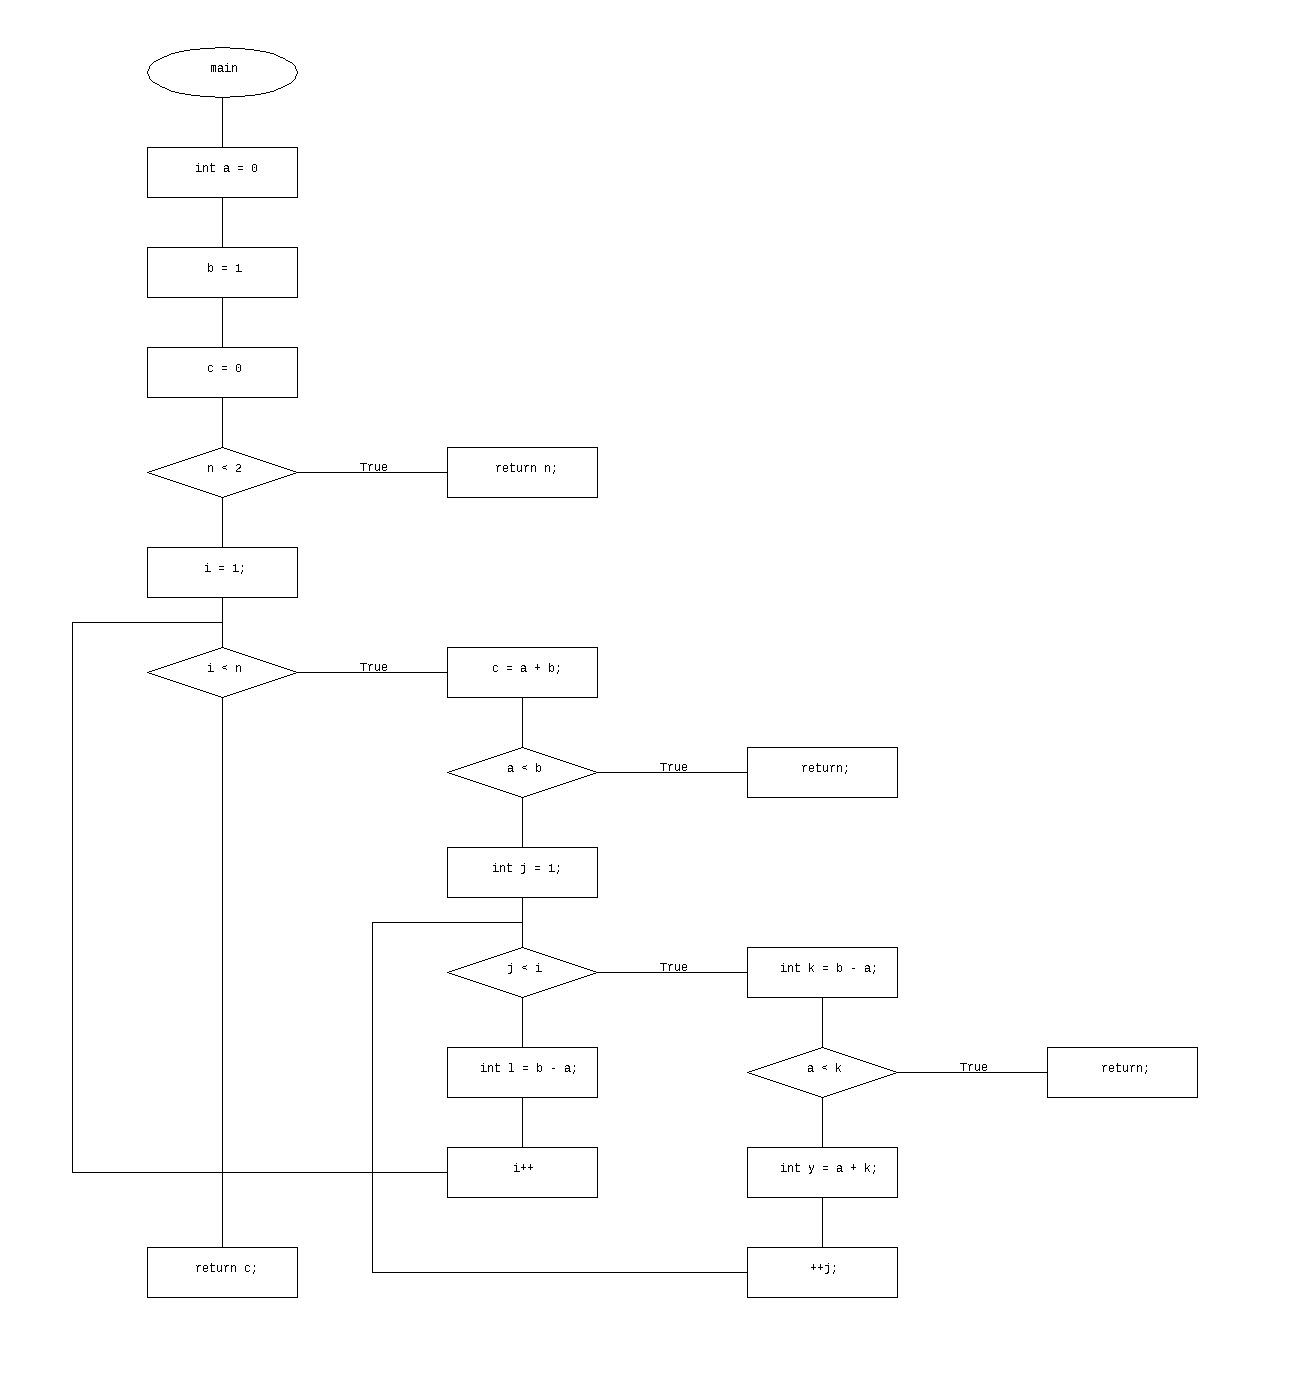
\includegraphics[scale=0.4]{test}
		\caption{Тестовый пример} 
		\label{pic:test} % название для ссылок внутри кода
	\end{center}
\end{figure}

\newpage
\subsection{Выводы}

\end{document}
